\documentclass[12pt]{article}
\usepackage[T2A,T1]{fontenc}
\usepackage[utf8]{inputenc}
\usepackage[english,russian]{babel}
\usepackage[14pt]{extsizes}

\usepackage{ucs}


\usepackage{amsmath}
\usepackage{amssymb}
\usepackage{float}
\usepackage{graphicx}
\usepackage{tikz}
\usepackage{titlesec}
\usepackage{misccorr}
\usepackage{indentfirst}
\usepackage{hyperref}
\usepackage{multirow}
\usepackage{tocloft}

\usepackage{soulutf8}
\newcommand{\cmt}[1]{\hl{ #1 }}
\newcounter{c_tab}
\setcounter{c_tab}{0}
\newcommand{\tabn}{\arabic{c_tab}}
\newcommand{\nextline}{\tabularnewline\hline}
\newcommand{\Table}[5][numbered]{\par\vspace{-0.1cm}\begin{flushright}\ifthenelse{\equal{#1}{numbered}}%
		{\addtocounter{c_tab}{+1}{\footnotesize\textbf{Таблица\,\,\tabn.} #2}}%
		{{\footnotesize\textbf{Таблица.} #2}}%
	\end{flushright}\vspace{-0.5cm}\par{\footnotesize\begin{center}\begin{tabular}{#3}\hline#4\end{tabular}\end{center}}}%
\usepackage{algorithm}
\usepackage[noend]{algpseudocode}

\usepackage{pgfplots}

\usepackage{statmodtitle}

\selectlanguage{russian}


\usetikzlibrary{shapes,arrows,positioning}

\topmargin=-1.0cm
\setlength{\textheight}{23,7cm}
\setlength{\textwidth}{15cm}
\hoffset=-10mm
\voffset=-10mm


\university{Санкт-Петербургский государственный университет}
\author{Ашихмина Алёна Сергеевна}
\title{Определение семантической связности \\ документов на примере договоров}
\facility{Кафедра технологии программирования}
\spec{Направление Фундаментальная информатика и информационные технологии}
\supervisor{старший преподаватель Мишенин~А.Н.}
\chief{к.ф.-м.н., доцент Блеканов~И.С.}
\city{Санкт-Петербург}
\date{2018}

\begin{document}
\maketitle{}

\topmargin=-1.0cm
\setlength{\textheight}{20cm}
\setlength{\textwidth}{16cm}
\hoffset=-5mm
\voffset=10mm
\parindent=12mm

\newpage
\tableofcontents
\newpage



\section{Введение}
За последние десятилетия накопилось огромное количество данных, имеющих различное происхождение, вследствие чего появилась возможность проанализировать эти данные, а результаты использовать в образовании, науке и безопасности, а также для описания объектов или улучшения качества какой-либо продукции. Это можно сделать с помощью машинного обучения. 

К такого рода задачам относится поиск несоответствий в деловых документах. В качестве документов в данной работе рассматриваются государственные контракты. Все они построены по одному и тому же шаблону и имеют определенную семантическую структуру. Люди, которые работают с подобными документами, легко могут предсказать по предыдущей части документа следующую. Иногда в таких документах встречаются случаи мошенничества, опечатки и технические ошибки, например, как описанные в \cite{vedomosti,fontanka}, так называемые «аномалии». 

Необходимо научиться автоматически, проанализировав большой корпус «честных» документов на предмет их внутренней связности, определять такого рода аномалии. В качестве таких аномалий могут выступать документы или части документов, которые расходятся с общепризнанными шаблонами.
Учитывая объемы данных, которые каждая компания накопила на сегодняшний день, и которые продолжает генерировать, причем всё в больших размерах, можно сделать вывод, что рассматриваемая задача становится исключительно актуальной. Вследствие чего в данной работе будут предложены несколько подходов к семантическому анализу текста. 

\newpage
\section{Постановка задачи}
Имеется коллекция документов (контрактов) $$D = \{d_1,\ldots,d_i,\ldots,d_n\}$$

Целью является разработка алгоритма, который позволил бы обобщать семантическую структуру документа и по контексту определять аномальность конкретного блока в договоре, где под контекстом подразумевается текст, который находится вокруг наблюдаемого блока. Исходя из такой цели, были поставлены следующие задачи.
\par\begin{enumerate}{
	\vspace{-0.2cm}\item Собрать достаточное количество тренировочных данных. 
	\vspace{-0.2cm}\item Обработать и подготовить к дальнейшему анализу, в том числе отфильтровать. 
	\vspace{-0.2cm}\item Представить каждый документ $d_i$ в виде последовательности текстовых блоков $(d_{i1}, \ldots, d_{ik}, \ldots, d_{im})$. В качестве блоков можно использовать:
	\par\begin{itemize}{
				\vspace{-0.2cm}\item Фактические параграфы, которые доступны из метаданных документа (например, разбивка по секциям в \textit{MS Word}).
				\vspace{-0.2cm}\item Параграфы, полученные с помощью алгоритма TextTiling  \cite{texttiling}.
	}\end{itemize}
	\vspace{-0.2cm}\item Протестировать несколько подходов:
	\par\begin{itemize}{
			\vspace{-0.2cm}\item Бинарная классификация на основе модели LDA.
			\vspace{-0.2cm}\item Бинарная классификация на основе нормализации векторного представления.
			\vspace{-0.2cm}\item Бинарная классификация на основе предложенной в этой работе тематической модели.
			\vspace{-0.2cm}\item Анализ статистических данных, полученных после аннотации документов с использованием тематической модели.
	}\end{itemize}
	\vspace{-0.2cm}\item Оценить качество рассматриваемых подходов.
}\end{enumerate}

\newpage
\section{Обзор литературы}
Качественное описание алгоритма Latent Dirichlet Allocation можно увидеть в работе Дэвида Блея \cite{lda}, статья опубликована в 2003 году, но все-равно актуальная сейчас. Для ее построения, а также построения векторного представления слов, использовалась библиотека gensim \cite{gensim}. Про оба эти способа очень доступно написано в статье <<Сравнительный анализ методов word2vec и GloVe и некоторые выводы из него>> \cite{maslovskaya}.

С алгоритмом textilng помогла разобраться статья <<TextTiling: \linebreak Segmenting Text into Multi-paragraph Subtopic Passages>> \cite{texttiling}. В ней описывается алгоритм на уровне идеи, что идеально подходит для первичного ознакомления и погружения в предметную область. 

Для обработки текстовой информации львиную долю работы на себя взяли такие библиотеки, как nltk и pymorphy. Классификация и кластеризация произведена с помощью встроенных функций из инструмента scikit-learn.


\newpage
\section{Подготовка данных}
Договоры были предоставлены компанией «Диджитал Дизайн» \cite{dd} в виде документов в различных форматах, а именно .doc, .docx. Эти договоры находятся в открытом доступе, с ними можно ознакомиться на официальном сайте единой информационной системы в сфере закупок \cite{zakupki}. Для облегчения дальнейшей работы с полученными документами написана программа для извлечения необходимых данных из файлов разных форматов. 

%%\Figure{1\textwidth}{images/im1.eps}{Пример документа\label{im1}}
\vspace{5pt}
\begin{figure}[h]
	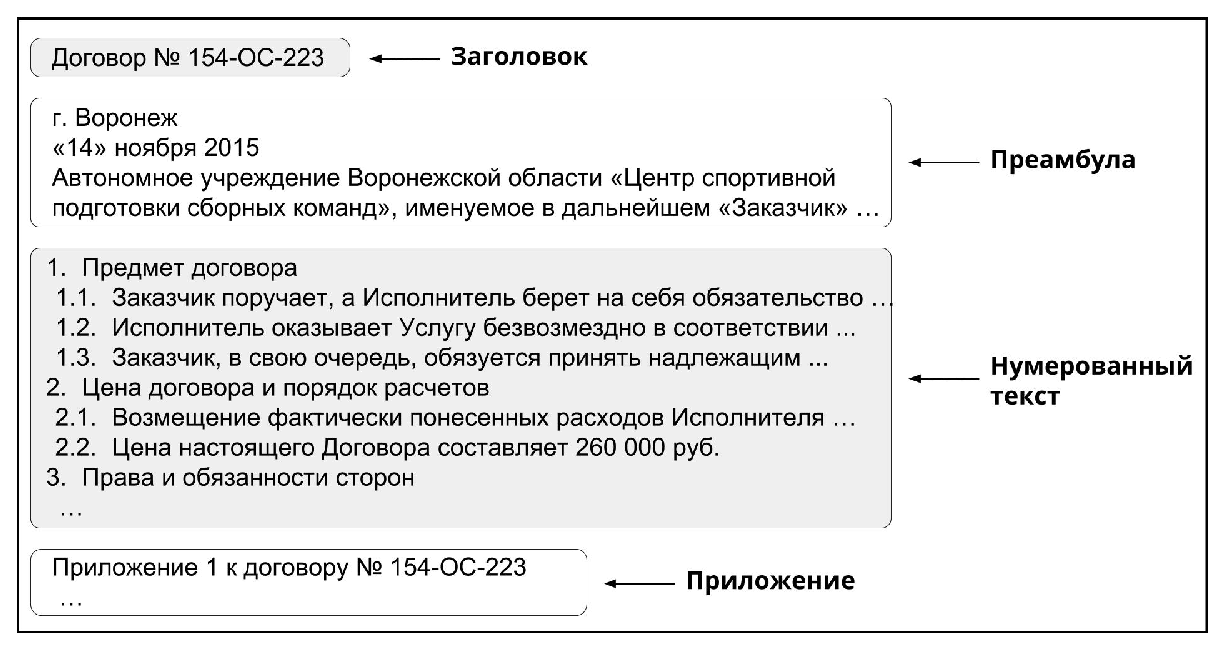
\includegraphics[scale=0.74]{images/im1.eps}
	\caption{Пример документа}
	\label{im1}
\end{figure}
\vspace{5pt}

В первую очередь была выявлена структура всего документа. После такой предобработки были выделены следующие сущности: Document, Paragraph и Sentence. Document хранит в себе информацию обо всем договоре и состоит из экземпляров Paragraph. Сущность Paragraph в свою очередь содержит информацию про каждый параграф (такими сущностями являются заголовок, преамбула, пункты договора и приложения) и состоит из предложений (экземпляров Sentence). Пример типичного договора представлен на рис.~\ref{im1}. 

\vspace{5pt}
\begin{figure}[h!]
	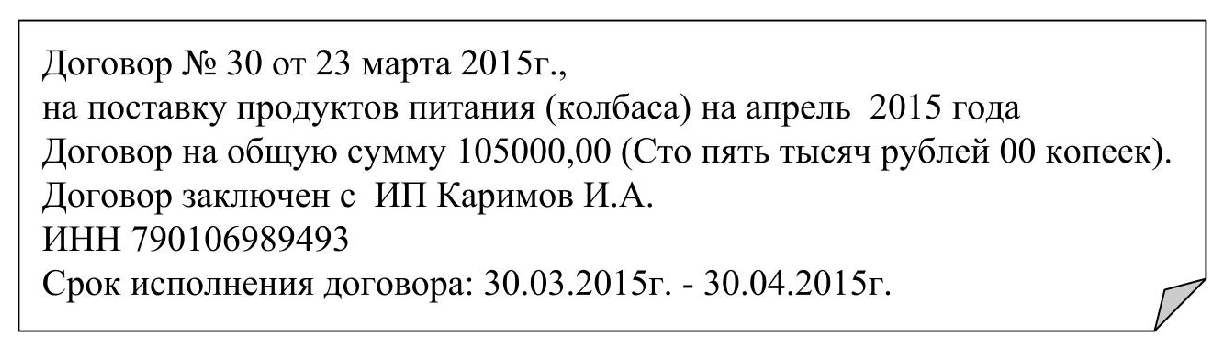
\includegraphics[scale=0.74]{images/im2.eps}
	\caption{Пример удаленного из коллекции документа}
	\label{im2}
\end{figure}
\vspace{5pt}

В коллекции присутствовали договоры разного вида, в том числе были такие, в которых не удалось обнаружить ни одной главы или обнаруженных параграфов было очень мало, поэтому от этих текстовых документов пришлось избавиться, чтобы они никак не повлияли \linebreak на результаты работы. Пример такого рода документа представлен на рис.~\ref{im2}.

Далее была проведена обработка текстовых данных для их дальнейшего применения, которая состоит из нескольких этапов.

\vspace{5pt}
\textbf{\textit{Токенизация}} - это разбиение текста на токены, в нашем случае токенами являются слова и числа. Полученные токены переводятся в нижний регистр, и с помощью регулярных выражений определяются  слова, состоящие из символов латинского алфавита и кириллицы,  а также было решено оставить для анализа числа, но заменить их на одну и ту же цифру “1”. Такая манипуляция с числовыми значениями позволит учитывать наличие каких-либо цифр как признак в тексте. 

Так, например, из такого предложения:

\vspace{13pt}
\noindent\textit{'Покупатель в срок не позднее 3 дней направляет Поставщику уведомление.'}

\vspace{13pt}
\noindent получится:

\vspace{13pt}
\noindent[\textit{'покупатель', 'не', 'позднее', '1', 'дней', 'направляет', 'поставщику', 'уведомление'}].

 \vspace{13pt}

Удаление \textbf{\textit{стоп-слов}} - слов, которые являются местоимениями или служебными частями речи, например, предлоги, союзы, частицы и так далее, такие слова встречаются почти в каждом предложении и не несут в себе смысловой информации. Для этого использовалась готовая коллекция слов библиотеки NLTK. 

Для рассмотренного выше примера получаем:

\vspace{13pt}
\noindent[\textit{'покупатель', 'позднее', '1', 'дней', 'направляет', 'поставщику', 'уведомление'}].
\vspace{13pt}

\textbf{\textit{Нормализация}} - приведение слова к начальной форме. На этом шаге использовалась библиотека pymorphy. Из предыдущего примера получим:

\vspace{13pt}
\noindent[\textit{'покупатель', 'поздний', '1', 'день', 'направлять', 'поставщик', 'уведомление'}].
\vspace{13pt}

Далее был проведен анализ получившихся договоров. Стало заметно, что слова, которые встречаются во всей коллекции менее 5 раз определенно являются либо опечатками, либо сокращениями, либо настолько специфичными, что рассматривать их нет смысла: 

\vspace{10pt}
\noindent\textit{'обезжелезивание', 'заболотья', 'барокко', 'госморспасслужба', 'разраб', 'фцп', 'перербург', 'обязонность', 'сссср'} и~т.~д.
\vspace{10pt}

Поэтому такие слова были исключены. Также было принято решение исключить слова, являющейся одной буквой, так как такие слова попали в коллекцию из инициалов и не несут в себе смысловой информации.

Еще, оказалось, что рассматривать в качестве блоков фактические параграфы не оптимально, так как они имеют очень разную длину. Поэтому для того, чтобы сделать их более однородными, а именно близкими по длине (количеству слов), в каждом документе последовательные параграфы были объединены таким образом, что в результате параграф имел длину не более 100 слов. Также было решено удалить из рассмотрения те документы, в которых получилось слишком мало параграфов, а именно меньше 5. Каждый такой параграф теперь рассматривается как текстовый блок, который может быть типичным или аномальным. 

В этой работе использовались данные, из которых можно было выявить естественное разделение документов на параграфы. Но, к сожалению, такая возможность есть не всегда. В таких случаях требуется самостоятельно проанализировать тексты и разбить каждый из них на части по какому-то признаку. С такой проблемой справляется TextTiling.

\textbf{\textit{TextTiling}} - это алгоритм разбиения текста на последовательность блоков, принадлежащих разным темам. Предполагается, что во время обсуждения одной темы используется определенная лексика, и когда эта тема меняется, значительная часть словарного состава также меняется. Texttiling предназначен для распознавания границ так называемых блоков, путем определения мест, где происходят максимальные изменения тем.
Этот алгоритм состоит из трёх основных частей:
\par\begin{enumerate}{
		\vspace{0.2cm}\item Токенизация
		
		На этом этапе все слова переводятся в нижний регистр, стоп-слова удаляются, каждое слово приводят в начальную форму (выделяют корень). Далее текст разделяется на псевдопредложения длиной w (параметр алгоритма), а не на реальные синтаксически определенные предложения. Это делается для дальнейшего сравнения количества общих терминов, так как сопоставление двух одинаково длинных предложений и сопоставление короткого и длинного дадут разные результаты. Информация о местах и количестве вхождений каждого токена в псевдопредложения после такой обработки сохраняется для дальнейшего анализа.
		
		\vspace{0.2cm}\item Определение лексической оценки (The lexical score)
		
		\par\begin{itemize}{
				\item С помощью блоков (Blocks).
				
				Согласно этому методу смежные пары блоков сравниваются с целью нахождения их лексического подобия. Размер блока $k$ представляет собой количество объединенных последовательных псевдопредложений. Это значение предназначено для аппроксимации средней длины так называемого абзаца (фактические абзацы не используются ввиду их нерегулярных длин, что приводит к несбалансированным сравнениям). Пусть есть два блока:
				
				\begin{center}
					$b_1 = \{token$-$sequence_{i-k}, \ldots, token$-$sequence_i\},$ 
					$b_2 = \{token$-$sequence_{i+1}, \ldots, token$-$sequence_{i+k+1}\},$ 
				\end{center}
				\noindent где $token$-$sequence_i$ - псевдопредложение, состоящее из токенов.
				
				Тогда для каждой пары последовательных блоков вычисляется величина их подобия таким образом: 
				
				$$score(i) = \frac{\sum_{t}(w_{tb_1}w_{tb_2})}{\sqrt{\sum_{t}(w_{tb_1}^2)\sum_{t}(w_{tb_2}^2)}},$$
				
				$t$ пробегает по всем токенам из словаря, $w_{tb}$ - вес термина $t$ в блоке $b$ (частота термина в блоке).
				
				\vspace{0.2cm}\item C помощью оценки словаря (Vocabulary Introduction).	
				
				В этом методе также рассматриваются два блока $b_1$, $b_2$:
				
				\begin{center}
					$b_1 = \{tokens_{i-w}, \ldots, tokens_i\},$ 
					$b_2 = \{tokens_{i+1}, \ldots, tokens_{i+w+1}\}$. 
				\end{center}
					
				Следует заметить, что теперь блоки составляют последовательность токенов, то есть псевдопредложение длиной $w$, в то время как в предыдущем методе под блоком подразумевалась последовательность из $k$ псевдопредложений. 
				
				Оценка высчитывается как отношение количества новых слов в интервале к длине всего интервала:
				
				\begin{center}
				$$score(i) = \frac{NumNewTerms(b_1) + NumNewTerms(b_2)}{w^2},$$
				\end{center}
				\noindent где $NumNewTerms(b)$ - количество терминов в блоке $b$, которые встретились в тексте в первый раз.
		}\end{itemize}
	
		\vspace{0.2cm}\item Определение границ
		
		На этом этапе одинаково для обоих методов лексической оценки определяется глубина разрыва на стыках каждой пары псевдопредложений. Под глубиной имеется в виду насколько сильно меняется речь с обеих сторон от рассматриваемого разрыва, то есть расстояние от пиков по обе стороны разрыва до него. Таким образом, если разрыв находится в относительно более глубокой долине, то он получает более высокие оценки границ, чем те, что расположены в менее глубоких долинах. 
		
		Более формально это можно сформулировать таким образом: рассматриваем разрыв $i$. Программа последовательно рассматривает лексическую оценку разрывов слева от $i$-го: $i-1$, $i-2$, \ldots, до тех пор пока не дойдет до разрыва $l$, такого, что $score(i-l-1) < score(i-l)$. Аналогично для разрывов справа от $i$-го: $i+1$, $i+2$, \ldots находит разрыв $r$, такой что $score(i+r+1) < score(i+r)$. 
		
		И, наконец, получаем значение глубины: 
		\begin{center}
			$depth$-$score(i) = [score(r) - score(i)] + [score(l) - score(i)].$ 
		\end{center}
		
		Таким образом величина глубины в точке $a_2$, изображенной на рис. 3(а), вычисляется как $score(a_1) - score(a_2) + score(a_3) - score(a_2)$.
		
		\vspace{5pt}
		\begin{figure}[h!]
			\center{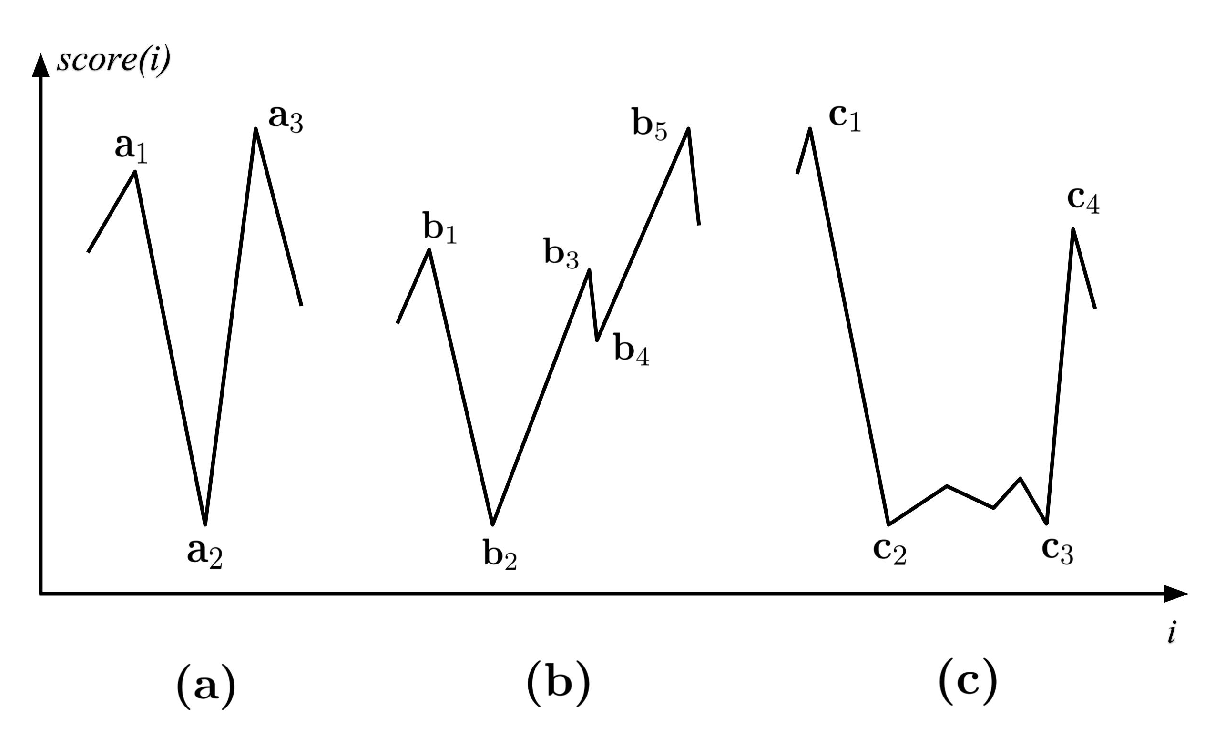
\includegraphics[scale=0.64]{images/im3.eps}}
			\caption{$score(i)$}
			\label{im3}
		\end{figure}
		\vspace{5pt}
		
		У такого подхода существует ряд потенциальных проблем, изображенных на рис. 3(b) и 3(c). В первом случае мы видим небольшую долину, которая затрудняет оценку для $b_2$. В качестве меры защиты алгоритм использует сглаживание, чтобы устранить небольшие возмущения, как $b_4$. Кроме того, расстояние между $b_3$ и $b_4$ невелико, поэтому этот промежуток с меньшей вероятностью будет рассмотрен как граница, чем, например, границы, которые окружают $b_2$. 
		
		Ещё одна проблема, изображенная на рисунке 3(c), возникает, когда два достаточно сильных пика расположены вдоль длинной плоской долины. В этом случае необходимо решить, где именно должна быть назначена граница: в $c_2$, $c_3$ или в них обоих. Такое <<плато>> возникает, когда речь меняется постепенно, и указывает на частично плохое соответствие построенной модели и документа. Когда плато имеет место на длинном участке, следует в качестве границ брать оба значения. Однако, если это длится не долго, то алгоритм вынужден произвольно выбрать одну из вершин. 
		
		После вычисления всех значений глубины, они сортируются и далее используются для определения границ: чем выше оценка, тем вероятнее, что граница находится в этом месте (по возможности корректируя границы, для того, чтобы они совпали с границами фактических абзацев, если такая возможность есть). Также предполагается, что между границами должны находиться не менее трех псевдопредложений.
}\end{enumerate}


Таким образом в результате проделанной предобработки тексты были разделены на блоки и сериализованы в бинарный формат.

\subsection{Подготовка тестовых данных}
Поскольку документы не искусственно сгенерированы, а, наоборот, являются настоящими договорами, то необходимо в данные добавить аномалии. Для этого в некоторой выборке документов блоки были равномерно заменены на случайные блоки из всей коллекции. Таким образов, случайно подменив некоторые блоки в документах на другие, которые выпадают из контекста и являются аномальными, мы искусственно получили данные для обучения и тестирования наших моделей. Цель свелась в построении алгоритма для определения этих подмешенных параграфов. Фактически в тестовой выборке получилось  12\% "аномальных" параграфов.

В конечном итоге был получен корпус из 9867 документов-договоров, которые составляют 210759 параграфов, 25203 из которых аномальные. Средняя длина параграфа получилась 89 слов.

\newpage
\section{Описание методов}
\subsection{LDA}
В первую очередь было решено опробовать тематическую модель LDA (latent Dirichlet allocation) - это генеративная статистическая модель, согласно которой, считается, что темы в документах подчиняются закону распределению Дирихле, а каждому текстовому блоку ставится в соответствие вектор, состоящий из вероятностей того, что данный блок принадлежит соответствующей теме. Для построения модели была написана программа на языке python с помощью библиотеки gensim []. Число тем, полученное после построения модели, сначала варьировалось, но позже эмпирически было выбрано количество 10. 
Пример представления полученных 10 тем при помощи 3 различных слов из словаря, собранного со всей коллекции, представлен в таблице 1. Можно заметить, что темы достаточно показательные, и слова, соответствующие конкретной теме, характеризуют нечто похожее по своей природе. 

\Table{Пример представления полученных 10 тем}{|p{1cm}|p{12cm}|}{
	\centering\textbf{№ темы} & \centering{\textbf{Тема}} \nextline
	\centering 1 & \centering{$0,\!032\times \text{<<обязательный>>} + 0,\!030\times \text{<<рубль>>} + 0,\!030\times \text{<<цена>>}$} \nextline
	\centering 2 & \centering{$0,\!116\times \text{<<товар>>} + 0,\!051\times \text{<<поставщик>>} + 0,\!032\times \text{<<поставка>>}$} \nextline
	\centering 3 & \centering{$0,\!089\times \text{<<работа>>} + 0,\!060\times \text{<<заказчик>>} + 0,\!043\times \text{<<подрядчик>>}$} \nextline
	\centering 4 & \centering{$0,\!086\times \text{<<сторона>>} + 0,\!043\times \text{<<договор>>} + 0,\!037\times \text{<<настоящий>>}$} \nextline
	\centering 5 & \centering{$0,\!033\times \text{<<карта>>} + 0,\!029\times \text{<<уп>>} + 0,\!020\times \text{<<работник>>}$} \nextline
	\centering 6 & \centering{$0,\!090\times \text{<<договор>>} + 0,\!047\times \text{<<настоящий>>} + 0,\!040\times \text{<<приложение>>}$} \nextline
	\centering 7 & \centering{$0,\!053\times \text{<<запрос>>} + 0,\!046\times \text{<<электронный>>} + 0,\!043\times \text{<<котировка>>}$} \nextline
	\centering 8 & \centering{$0,\!046\times \text{<<договор>>} + 0,\!035\times \text{<<услуга>>} + 0,\!033\times \text{<<заказчик>>}$} \nextline
	\centering 9 & \centering{$0,\!051\times \text{<<договор>>} + 0,\!038\times \text{<<исполнение>>} + 0,\!029\times \text{<<обязательство>>}$} \nextline
	\centering 10 & \centering{$0,\!040\times \text{<<адрес>>} + 0,\!036\times \text{<<плата>>} + 0,\!031\times \text{<<рубль>>}$}\nextline
}


Полученные векторы необходимо было нормировать, и после этого можно было прислупать к классификации. Множество объектов было разделено на тренировочное и тестовое в соотношении 70:30, и, наконец, построен классификатор методом $k$ ближайших соседей. Построенная модель определяла неаномальный параграф как неаномальный в 99\% случаев, а вот аномальные параграфы как аномальные всего в 45\% случаев. Даже при увеличении объёма данных в 3 раза качество определения аномальных параграфов увеличилось всего до 47\%.


\subsection{Векорное представление слов}

Еще одним способом векторного представления имеющихся документов (<<word embedding>>) был выбран инструмент word2vec, который уже реализован в библиотеке gensim, хотя существует ещё несколько аналогичных ему моделей, например, Glove \cite{glove} или fastText \cite{fasttext}. Word2vec был выбран из сообGlove особое внимание уделяет статистическим данным, в отличие от word2vec, который не содержит в себе этапа предварительного сбора статистики \cite{zakirov, predict}. А в fastText, в отличие от word2vec, в котором минимальной единицей считается слово, используются n-граммы — последовательности из n символов слова. Согласно этой модели вектор слова является суммой входящих в него n-грамм.

В основе word2vec лежат два алгоритма: continuous bag of words (CBOW) и skip-gram. CBOW решает задачу предсказания слова по его контексту, а skip-gram - наоборот, по имеющемуся слову предугадывает слова, которые его окружают. По причине того, что этот инструмент построен на обучении нейронных сетей, его качество зависит от размера выбранной коллекции для обучения. Сервис RusVectōrēs предоставляет доступ всем желающим к различным корпусам документов на русском языке. Но в контексте данной работы было принято решение натренировать модель на имеющейся базе контрактов. Так как всё-таки задача была поставлена с чётким уклоном именно на договоры, а они имеют специфическую лексику, в то время как стилистика текстов из коллекций RusVectōrēs сильно разнообразна. Следовательно модель, обученная на таком множестве, может считать текстовые блоки очень схожими по значению, в то время как в контексте имеющейся коллекции они будут существенно отличаться. 

Итак, каждому слову модель ставит в соответствие его векторное представление. Но необходимо построить вектор, соответствующий текстовому блоку, в котором, как было написано выше, почти 100 слов. Поэтому было решено в качестве векторного представления текста считать сумму векторов его слов. Далее для каждого блока $b_i$ определили признаки таким же способом, как и в предыдущем подходе, а именно конкатенацией векторного представления предыдущего $b_{i-1}$, рассматриваемого $b_i$ и последующего $b_{i+1}$ блоков. 

Формально это выглядит таким образом:

\begin{center}
	$b_i \leftrightarrow (v_{b_{i-1}}, v_{b_i}, v_{b_{i+1}})$
\end{center}

На этот раз было решено рассмотреть коллекцию, в три раза превышающую предыдущую по размеру. Полученные векторы аналогично предыдущему подходу были стандартизированы, а объекты разделены на тренировочное и тестовое множества в сооношении 70:30 и на их основе был построен бинарный классификатор методом $k$ ближайших соседей.

Проанализируем полученные результаты:

\begin{table}[H]
	\centering
	\vspace{-0.5cm}
	\caption{Таблица контингентности}
	\vspace{0.2cm}
	\label{my-label}
	\begin{tabular}{|l|l|p{3cm}|c|}
		\hline
		\multicolumn{2}{|c|}{\multirow{2}{*}{}}                                      & \multicolumn{2}{c|}{Экспертная оценка} \\ \cline{3-4} 
		\multicolumn{2}{|c|}{}                                                       & \centering Аномалия                  &  Не аномалия \\ \hline
		\multirow{2}{*}{\begin{tabular}[c]{@{}l@{}}Оценка\\ модели\end{tabular}} & Аномалия & \centering TP                 &  FP                \\ \cline{2-4} 
		& Не аномалия & \centering FN                 & TN                \\ \hline
	\end{tabular}
\end{table}
\noindent где TP --- истинно-положительная оценка (true positive), 
TN --- истинно-отрицательная оценка (true negative), FP --- ложно-положительная оценка (false positive), FN --- ложно-отрицательная оценка (false negative).  
Для начала оценим значения ошибок 1-го и 2-го рода на сформированном выше тестовом множестве. В данном случае ошибкой 1-го рода является показатель FP, а 2-го рода - FN, проиллюстрированные в таблице 2. Они составляют соответственно 31\% и 0,001\%. 

Рассмотрим значения точности $precision$ и полноты $recall$:

\begin{center}
	$precision =  \frac{TP}{TP + FP} = 0,8963$, 
	
	$recall = \frac{TP}{TP + FN} = 0,6407$
\end{center}

\noindent а также функционал $F(precision, recall)$, который можно считать за усовершенствованную меру:

\begin{center}
	$F(precision, recall) =  \frac{2 \cdot precision \cdot recall}{precision + recall} = 0.7472$
\end{center}

Значения точности и полноты в процессе обучения должны увеличиваться, чем они выше, тем качественнее модель. При их увеличении значение функционала $F$ также будет увеличиваться, а при их стремлении к $0$ значение $F$ тоже будет стремиться к $0$. Это говорит о том, что использовать меру $F$ очень удобно, так как она совмещает в себе информацию и о точности, и о полноте.

Несмотря на такие, казалось бы, небольшие показатели, модель распознает 64\% аномальных параграфов как аномальные.

\subsection{Усовершенствованный подход на основе построенной тематической модели}
Ранее в работе в качестве векторного представления блока текста рассматривался усредненный вектор word2vec по словам, из которых состоит блок. Но такой способ векторизации текста сглаживает ярко выраженные признаки слов, входящих в него, следовательно ухудшает качество построенной модели. Поэтому было решено рассмотреть другой алгоритм получения векторного представления текста:
\par\begin{enumerate}{
		\vspace{-0.2cm}\item Каждый блок текста	$b = \{word_1, word_2, …, word_n\}$ представляется в виде суммы векторов, соответствующих входящим в него словам:
		
		\noindent $v(b) = v(word_1) +\ldots + v(word_n)$.
		
		\vspace{-0.2cm}\item Полученный вектор $v(b)$ нормализуем, получится $norm(v(b))$.
		\vspace{-0.2cm}\item Для каждого слова из блока рассматриваем его расстояние до вектора $norm(v(b))$.
		\vspace{-0.2cm}\item Выбираем $N_1$ слов из блока, максимально близких к $norm(v(b))$.
		\vspace{-0.2cm}\item Вычисляем взвешенную сумму этих векторов по косинусной мере, получится $weighted$-$mean$.
		\vspace{-0.2cm}\item Выбираем $N_2$ слов из всей коллекции, ближайших к $weighted$-$mean$. Эти слова и будут соответствовать рассматриваемому параграфу.  Преимущество такого способа выбора слов в том, что эти они не обязательно должны присуствовать в рассматриваемом параграфе. Эти слова являются своего рода аннотацией к нему.
		\vspace{-0.2cm}\item Сформируем множество слов, которые описывают таким образом всю коллекцию. Выберем из них $N_3$ слов.
		\vspace{-0.2cm}\item Построим модель кластеризации методом $k$-средних с $N_4$ кластерами. В качестве объектов рассмотрим векторное представление выбранных $N_3$ слов. Таким образом мы получим координаты $N_4$ центроидов.
		\vspace{-0.2cm}\item Теперь любому новому текстовому блоку можно сопоставить расстояние от его взвешенной суммы, которая может быть получена, если следовать алгоритму, в пункте 5, до центроидов построенного кластеризатора.
}\end{enumerate}

В результате был построен кластеризатор с $N_4 = 20$ кластерами, каждый из которых можно описать словами из выбранных ранее $N_3 = 2000$ слов. Проанализировав эти слова каждый кластер был вручную озаглавлен. На рисунке 4 продемонстрированы получившиеся кластеры. 

Теперь каждому текстовому блоку $b$ ставится в соответствие конкатенация векторов-расстояний от взвешенного среднего до центроидов.

\begin{center}
	$b_i \leftrightarrow (l_{i1}, l_{i2},\ldots, l_{i20})$
\end{center}

Как оценить такой подход?  

\subsection{Анализ статистических данных}
Теперь можно построить статистическую модель того, в каком порядке параграфы, принадлежащие разным темам, сменяют друг друга. В таблице 3 показаны вероятности в процентах $p_{ij}$, $i = 1,\ldots, 20$, $j = 1,\ldots, 20$ того, что тема $i$ сменится на тему $j$ при переходе от одного текстового блока к следующему.


\newpage

\section{Заключение}
В данной работе была поставлена цель разработать алгоритм, определяющий алогичность в деловых документах, предложено несколько подходов к решению поставленных задач. Было учтено, что данные, с которыми придется работать, не обязательно уже разбиты на осмысленные параграфы, в таких случаях можно самостоятельно разбить текст на блоки с помощью алгоритма texttiling. 

Было рассмотрено несколько способов векторного представления текстовых блоков. В рамках одного из подходов был построен классификатор, с помощью результатов которого появилась возможность явно обозначить темы, которые присущи текстам такого формата, как деловой контракт. 

Все предложенные подходы показали довольно достойные результаты. В работе не были учтены такие аномалии как нетипичные цены, например, сахар за миллион рублей и в процессе работы основывались только на тематических моделях. Поэтому в этой области осталось весьма широкое поле для экспериментов в сторону различных рекурентных нейронных сетей и отказа от принципа bag of words.

\newpage


\begin{thebibliography}{99}
\vspace{-7pt}

\bibitem{vedomosti} Заемщик переписал условия договора банка Тинькова [Электронный ресурс] // Ведомости.  \url{URL: https://www.vedomosti.ru/finance/articles/2013/08/07/zaemschik-perepisal-usloviya-dogovora-banka-tinkova-i} (дата обращения: 13.03.18).

\bibitem{fontanka} Сорок процентов --- откат нормальный. Пальчики оближешь [Электронный ресурс] // Фонтанка.  \url{URL: http://www.fontanka.ru/2018/01/15/110/} (дата обращения: 13.03.18).

\bibitem{lda} David~M.\:B., Andrew~Y.\:Ng., Michael~I. Latent Dirichlet allocation // Journal of Machine Learning Research. 1997. Vol.~3. P.~993--1022.

\bibitem{texttiling} Marti~A. Hearst TextTiling: Segmenting Text into Multi-paragraph Subtopic Passages // Computational Lingustics. 2003. Vol.~323. P.~33--64.

\bibitem{w2v} Deep learning with word2vec [Электронный ресурс]: \url{URL: https://radimrehurek.com/gensim/models/word2vec.html} (дата обращения: 14.03.18).

\bibitem{dd}  Digital Design [Электронный ресурс]: \url{URL: https://digdes.ru/} (дата обращения: 14.03.18).

\bibitem{zakupki} Портал закупок [Электронный ресурс]: \url{URL: http://zakupki.gov.ru/epz/main/public/home.html} (дата обращения: 14.03.18).

\bibitem{nltk} Natural Language Toolkit [Электронный ресурс]: \url{URL: https://www.nltk.org/} (дата обращения: 14.03.18).

\bibitem{vorontsov} Воронцов~К.\:В. Вероятностные тематические модели коллекций текстовых документов [Электронный ресурс]: \url{URL:  http://www.machinelearning.ru/wiki/images/c/c2/Vorontsov2apr2012.pdf} (дата обращения: 14.03.18).

\bibitem{gensim}  Gensim. Topic modelling for humans [Электронный ресурс]: \url{URL: https://radimrehurek.com/gensim/} (дата обращения: 14.03.18).

\bibitem{glove}  GloVe: Global Vectors for Word Representation [Электронный ресурс]: \url{URL: https://nlp.stanford.edu/projects/glove/} (дата обращения: 14.03.18).

\bibitem{fasttext}  FastText. Library for efficient text classification and representation learning [Электронный ресурс]: \url{URL: https://fasttext.cc/} (дата обращения: 14.03.18).

\bibitem{predict}   Marco~B., Georgiana~D., German~K. Don’t count, predict! A systematic comparison of context-counting vs. context-predicting semantic vectors //  Proceedings of the 52nd Annual Meeting of the Association for Computational Linguistics. 2014. Vol.~1. P.~238--247.

\bibitem{zakirov}  Закиров~М.\:А. Сравнительный анализ методов word2vec и GloVe и некоторые выводы из него // Современная наука: актуальные проблемы теории и практики. Серия: Естественные и технические науки. 2016. №~9--10. С.~36--41.

\bibitem{maslovskaya} Масловская М.\:А. Сравнение методов тематического моделирования // Процессы управления и устойчивость. 2017. T.~4. №~1. С.~423--427.

\bibitem{scikit}  Scikit-learn. Machine Learning in Python [Электронный ресурс]: \url{URL: http://scikit-learn.org/stable/} (дата обращения: 14.03.18).

\end{thebibliography}
\end{document}
